\subsection{Verifica MMS e bilanci}

Nella serie spaziale coordinata, gli errori $L^2$ decrescono per tutti i campi. Gli ordini empirici osservati sono circa 2.93--2.97 per lo spostamento, 2.02--2.06 per la pressione e 1.94--1.98 per il tracciante. Gli EOC in $H^1$ sono 1.98--1.99 per lo spostamento, 1.00--1.01 per la pressione e 1.40--1.71 per il tracciante. Questi ultimi valori indicano che il regime asintotico per la seminorma $H^1$ del tracciante non è stato dimostrato.

\begin{table*}[t]
\centering
\caption{Errori spaziali $L^2$ ed ordini di convergenza osservati (EOC) nella serie MMS coordinata. Il parametro $h=1/N$ è la larghezza della cella quadrata, non il diametro diagonale dell'elemento.}
\label{tab:spatial}
\small
\begin{tabular}{ccccccc}
\toprule
$h$ & $\|e_d\|_{L^2}$ & EOC & $\|e_p\|_{L^2}$ & EOC & $\|e_c\|_{L^2}$ & EOC\\
\midrule
0.2500 & $2.687\times10^{-3}$ & -- & $5.453\times10^{-3}$ & -- & $2.456\times10^{-2}$ & --\\
0.1250 & $3.529\times10^{-4}$ & 2.93 & $1.305\times10^{-3}$ & 2.06 & $6.396\times10^{-3}$ & 1.94\\
0.0625 & $4.493\times10^{-5}$ & 2.97 & $3.229\times10^{-4}$ & 2.02 & $1.616\times10^{-3}$ & 1.98\\
\bottomrule
\end{tabular}
\end{table*}

Nel raffinamento temporale con spazio $Q_2/Q_2/Q_2$, per $\Delta t_{\max}=0.05,0.025,0.0125,0.00625$, gli EOC dell'ultimo intervallo sono rispettivamente 1.06, 0.99 e 0.99 per $d,p,c$. Una diagnostica ulteriore, eseguita a mesh fissa e raddoppiando il numero di passi da 4800 a 9600, ha prodotto variazioni relative delle norme finali pari a 0.02\% per $d$, 0.75\% per $p$ e 3.24\% per $c$. Il contributo temporale per il tracciante non è quindi trascurabile in ogni regime; gli EOC della serie coordinata sono risultati osservati, non una prova isolata degli ordini spaziali teorici. Le tabelle complete sono riportate nell'Appendice A.

\begin{figure*}[t]
\centering
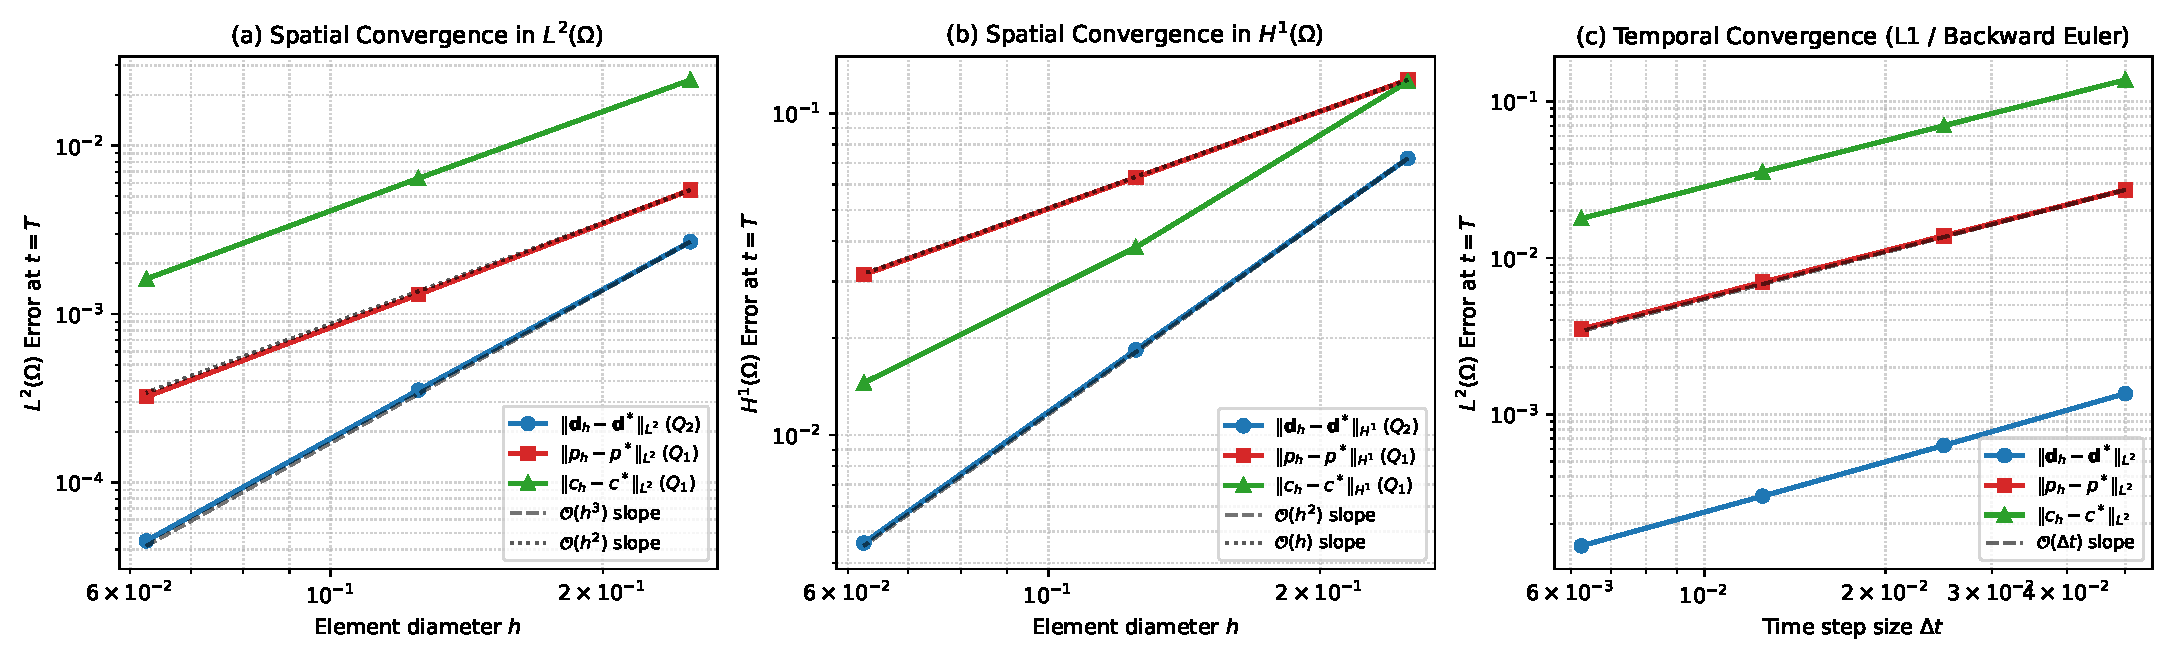
\includegraphics[width=0.94\textwidth]{paper/fig03_mms_convergence_complete.pdf}
\caption{Verifica MMS: errori spaziali $L^2$ e $H^1$ e raffinamento temporale $L^2$ per i tre campi. I tassi rappresentano il protocollo numerico eseguito; l'isolamento dell'errore spaziale richiede la cautela descritta nel testo.}
\label{fig:mms}
\end{figure*}

Sul quadrato, il residuo di compatibilità iniziale è $5.45\times10^{-16}$, l'errore massimo dell'identità algebrica passo-passo è $4.78\times10^{-17}$ e il drift relativo della massa del tracciante è $3.92\times10^{-15}$. Riducendo $\Delta t$ da 0.04 a 0.005, il residuo energetico cumulativo assoluto scende da $2.074\times10^{-3}$ a $2.903\times10^{-4}$. L'identità algebrica passo-passo è un controllo distinto dal residuo energetico cumulativo e non dimostra, da sola, una disuguaglianza energetica discreta generale.

\subsection{Geometria e campi della simulazione anatomica}

La maschera selezionata ha area $17069\,\mathrm{mm}^2$ e la mesh di riferimento area $17068.29\,\mathrm{mm}^2$, con errore relativo $4.17\times10^{-5}$, Dice rasterizzato 0.9982 e IoU 0.9963. Tutte le 1901 celle sono quadrilatere; non sono state rilevate celle invertite o degeneri. Questo conferma la fedeltà della mesh alla maschera definita, non la correttezza istologica della maschera. La forma anatomica è classificata come proxy del parenchima e non come sostanza bianca segmentata.

\begin{figure*}[t]
\centering
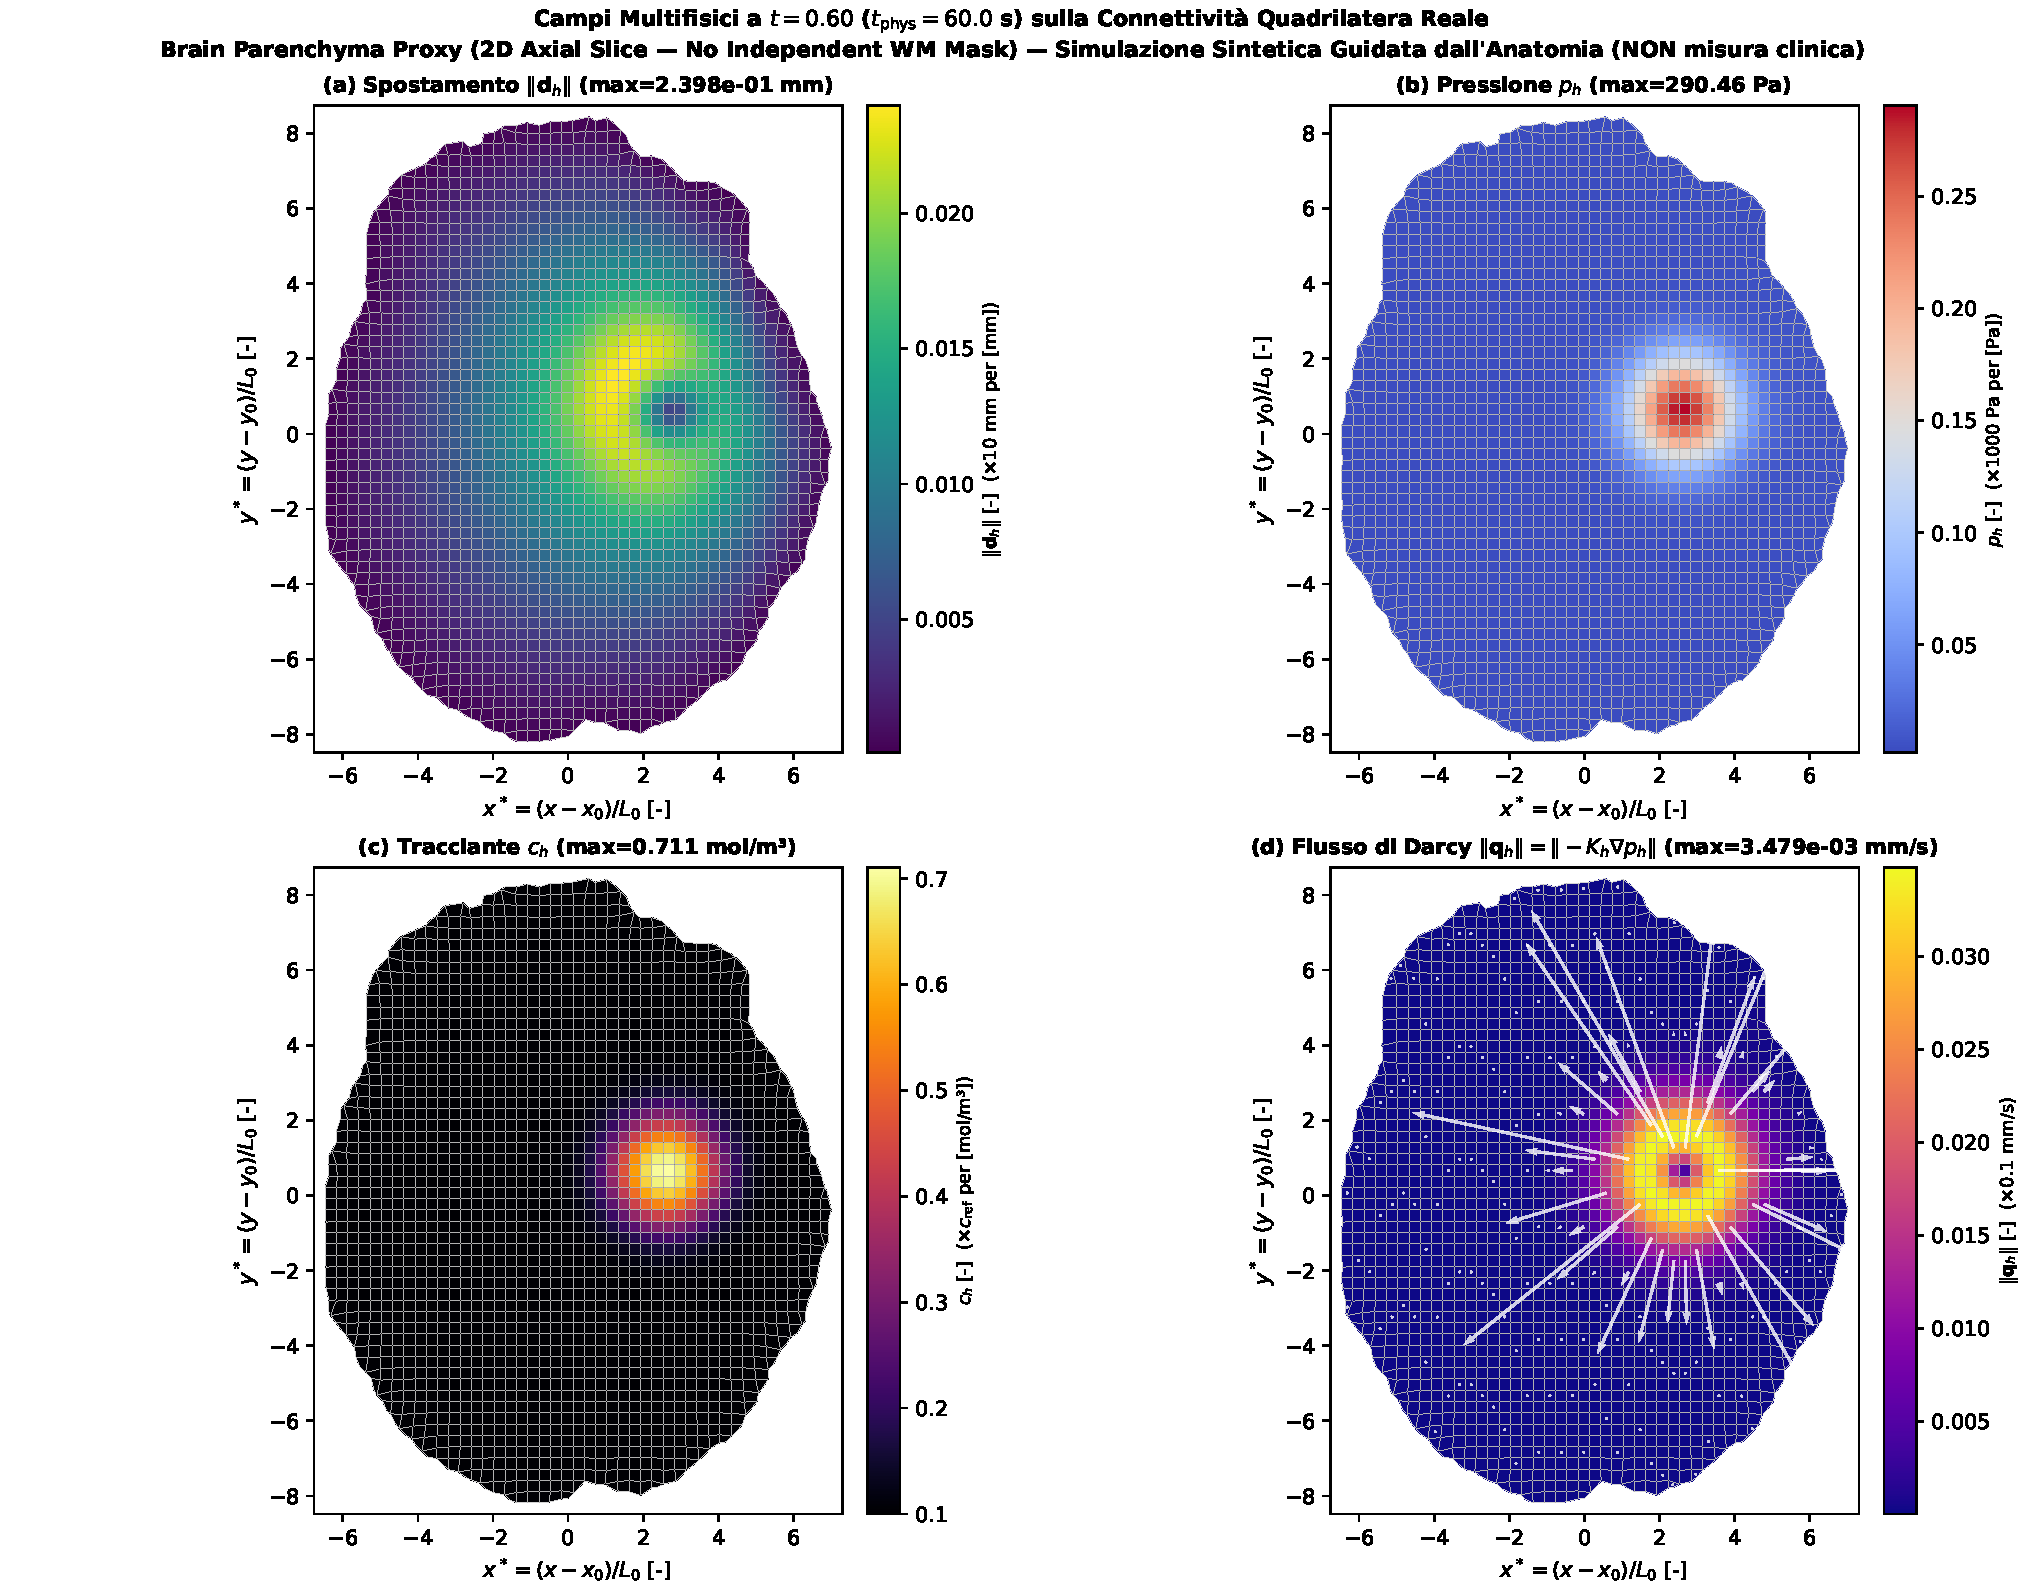
\includegraphics[width=0.94\textwidth]{paper/fig04_multiphysics_fields_on_quad_mesh.pdf}
\caption{Campi finali calcolati sulla connettività quadrilatera derivata dalla sezione BraTS. La sorgente è ancorata al centroide della lesione; ampiezze e andamenti temporali sono sintetici e non corrispondono a misure cliniche.}
\label{fig:fields}
\end{figure*}

La traiettoria anatomica ha norme finali adimensionali $\|d_h(T)\|_{L^2}=0.12105$, $\|p_h(T)\|_{L^2}=0.53803$ e $\|c_h(T)\|_{L^2}=1.97108$. La velocità di Darcy massima è 0.03678 adimensionale, equivalente a $3.68\times10^{-3}$ mm/s con le scale dichiarate. Sono statistiche della traiettoria forzata dal protocollo sintetico, non stime di variabili cliniche.

Il test di sensibilità alla mesh confronta dimensioni di lato obiettivo 4, 3 e 2 mm. Rispetto alla mesh da 2 mm, le differenze relative per la norma finale del tracciante sono 0.431\% (4 mm) e 0.186\% (3 mm); per la norma dello spostamento 0.562\% e 0.253\%; per l'energia totale finale 2.111\% e 0.895\%. Poiché non è disponibile una soluzione esatta sul dominio anatomico, tali differenze sono sensibilità alla discretizzazione, non ordini di convergenza. L'evoluzione temporale e le curve di sensibilità frazionaria sono raccolte nell'Appendice B.

\subsection{Conservazione e diagnostica energetica sulla mesh anatomica}

Sulla mesh da 3 mm, la massa adimensionale del tracciante passa da 21.08953037267824 a 21.089530372678244, con drift relativo massimo $6.74\times10^{-16}$. L'errore massimo dell'identità algebrica passo-passo è $7.65\times10^{-17}$. Al tempo finale, l'energia totale è 0.08551, la dissipazione viscoelastica cumulativa 0.00451, quella idraulica 0.01571 e il lavoro esterno cumulativo 0.10761; il residuo energetico cumulativo registrato è $-1.88\times10^{-3}$. Poiché i carichi sono attivi, l'energia totale non è attesa decrescere monotonicamente. Questi dati documentano il bilancio numerico del caso eseguito, non una prova generale della stabilità energetica dello schema.

\begin{figure*}[t]
\centering
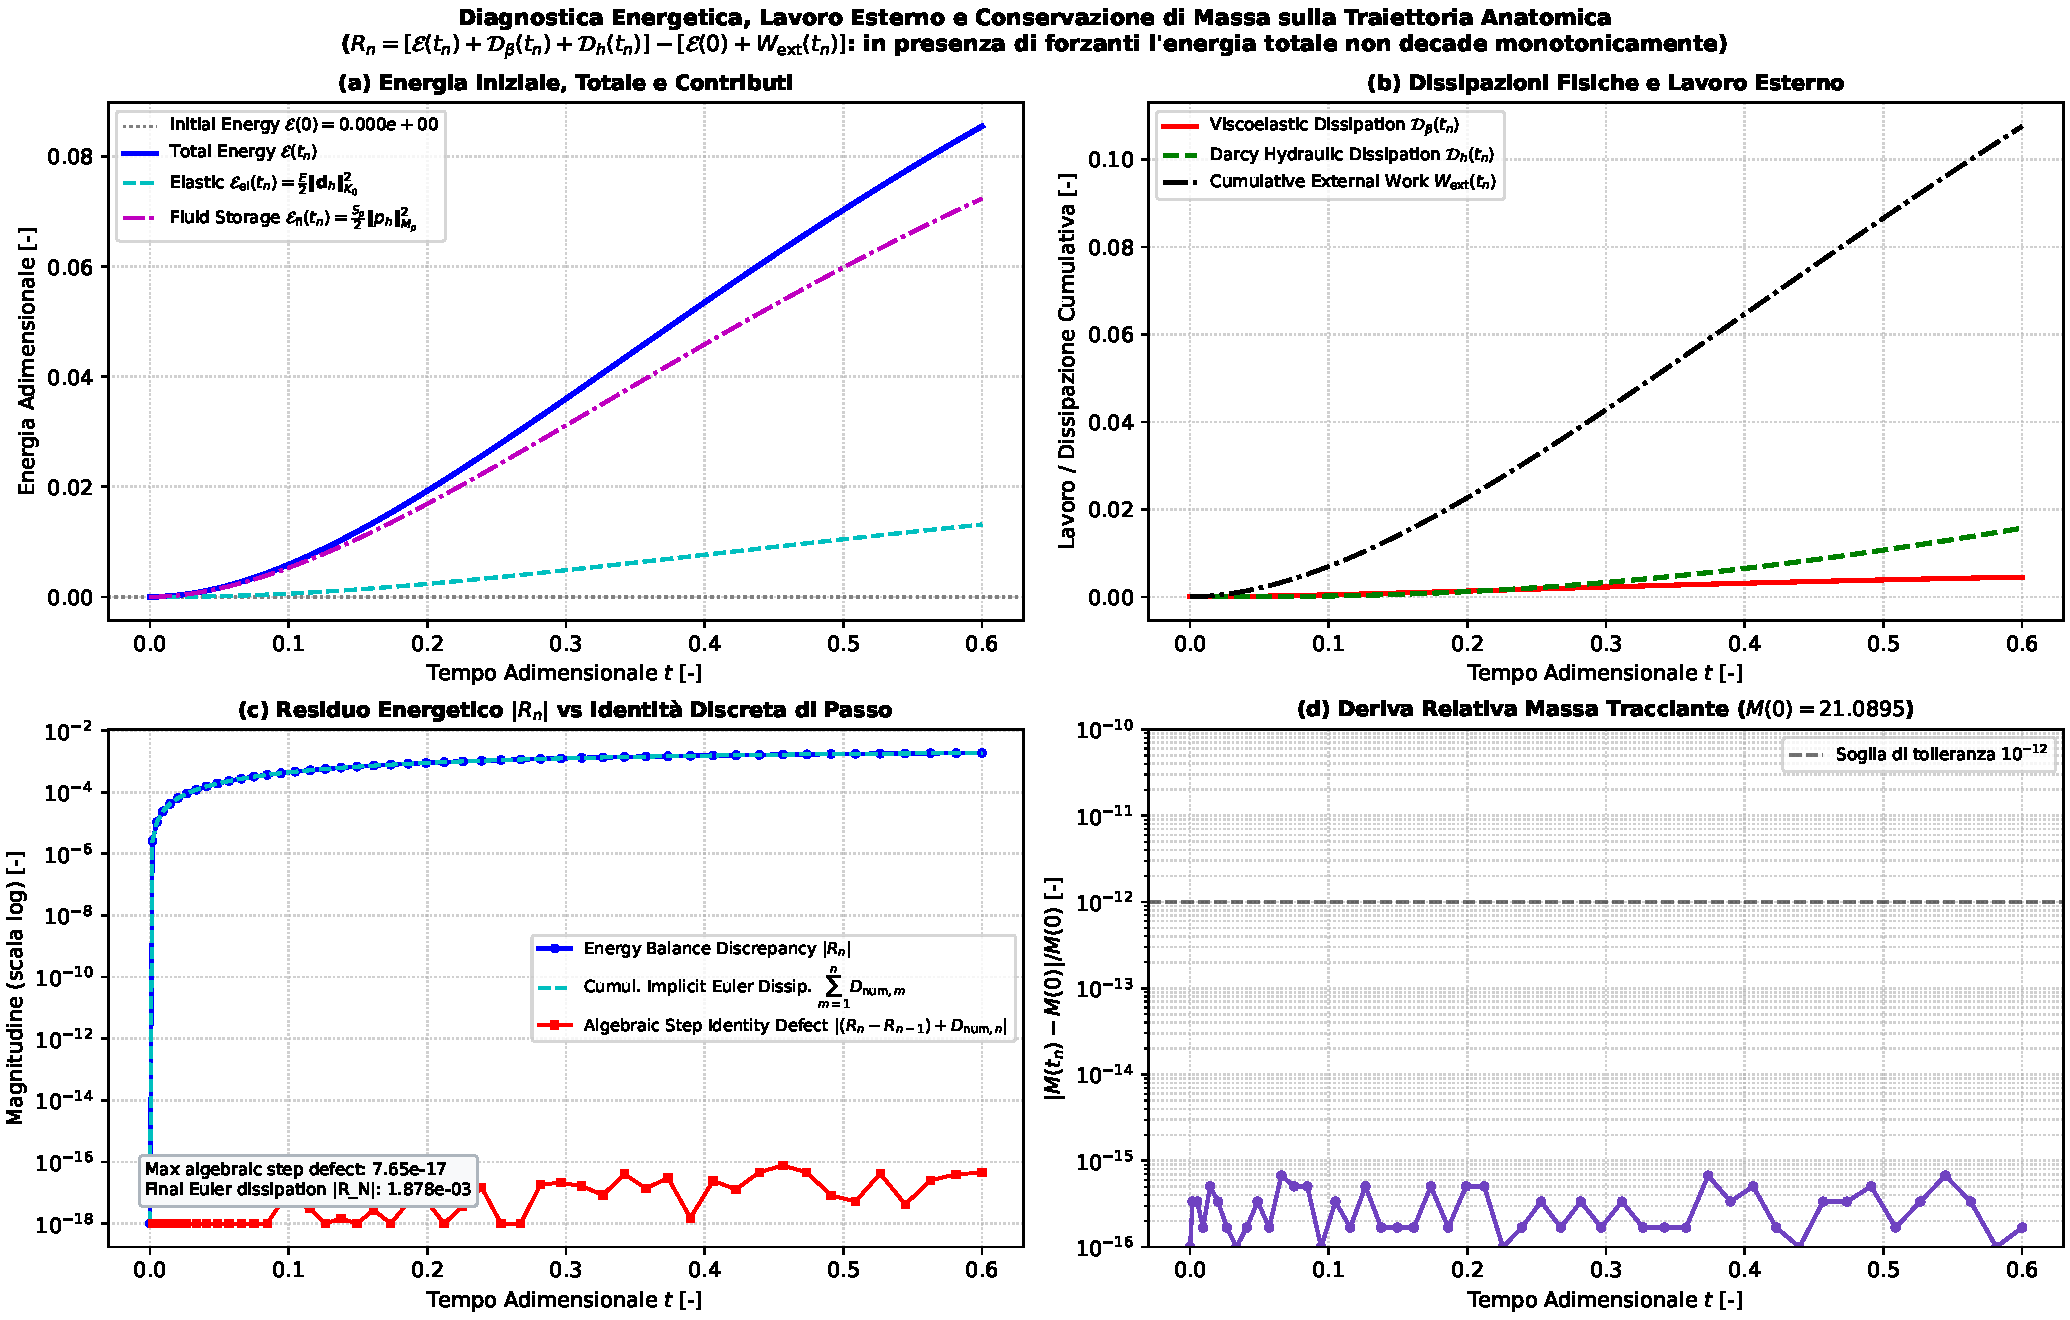
\includegraphics[width=0.94\textwidth]{paper/fig05_energy_and_mass_diagnostics.pdf}
\caption{Diagnostiche energetiche e di massa sulla traiettoria anatomica forzata. L'identità discreta passo-passo e il residuo globale sono mostrati come grandezze distinte.}
\label{fig:energy}
\end{figure*}

\subsection{Identificabilità locale: flusso nullo e flusso attivo}

Con sole osservazioni del tracciante, nel protocollo a flusso nullo tutte le nove traiettorie di perturbazione confermano $\mathbf q=0$, $p=0$ e $d=0$ entro la tolleranza configurata. Il Jacobiano discreto ha rango numerico 2: le colonne associate ad $\beta$ ed $E$ sono esattamente nulle e i valori singolari sono $(1.5833,0.3222,0,0)$. Questo è il riscontro numerico della Proposizione~\ref{prop:zeroq} nel protocollo testato.

Con il protocollo di carico attivo, il massimo della velocità di Darcy alla configurazione di riferimento è 0.05910 adimensionale e il Jacobiano ha rango numerico 4. I valori singolari sono $(1.2325,0.3784,0.3047,0.05229)$ e il numero di condizionamento è 23.57 secondo la convenzione del report. Il modo destro meno informativo è dominato da $\beta$ (componente circa $-0.9965$). La stabilità al passo di differenza finita è buona: variando il passo tra $10^{-3}$ e $10^{-5}$, la differenza relativa di Frobenius rispetto al Jacobiano di riferimento è al massimo $1.51\times10^{-6}$. Il rango pieno è evidenza di identificabilità locale regolare per quella mappa discreta e quel punto, non identificabilità globale né garanzia statistica di precisione.

\begin{figure*}[t]
\centering
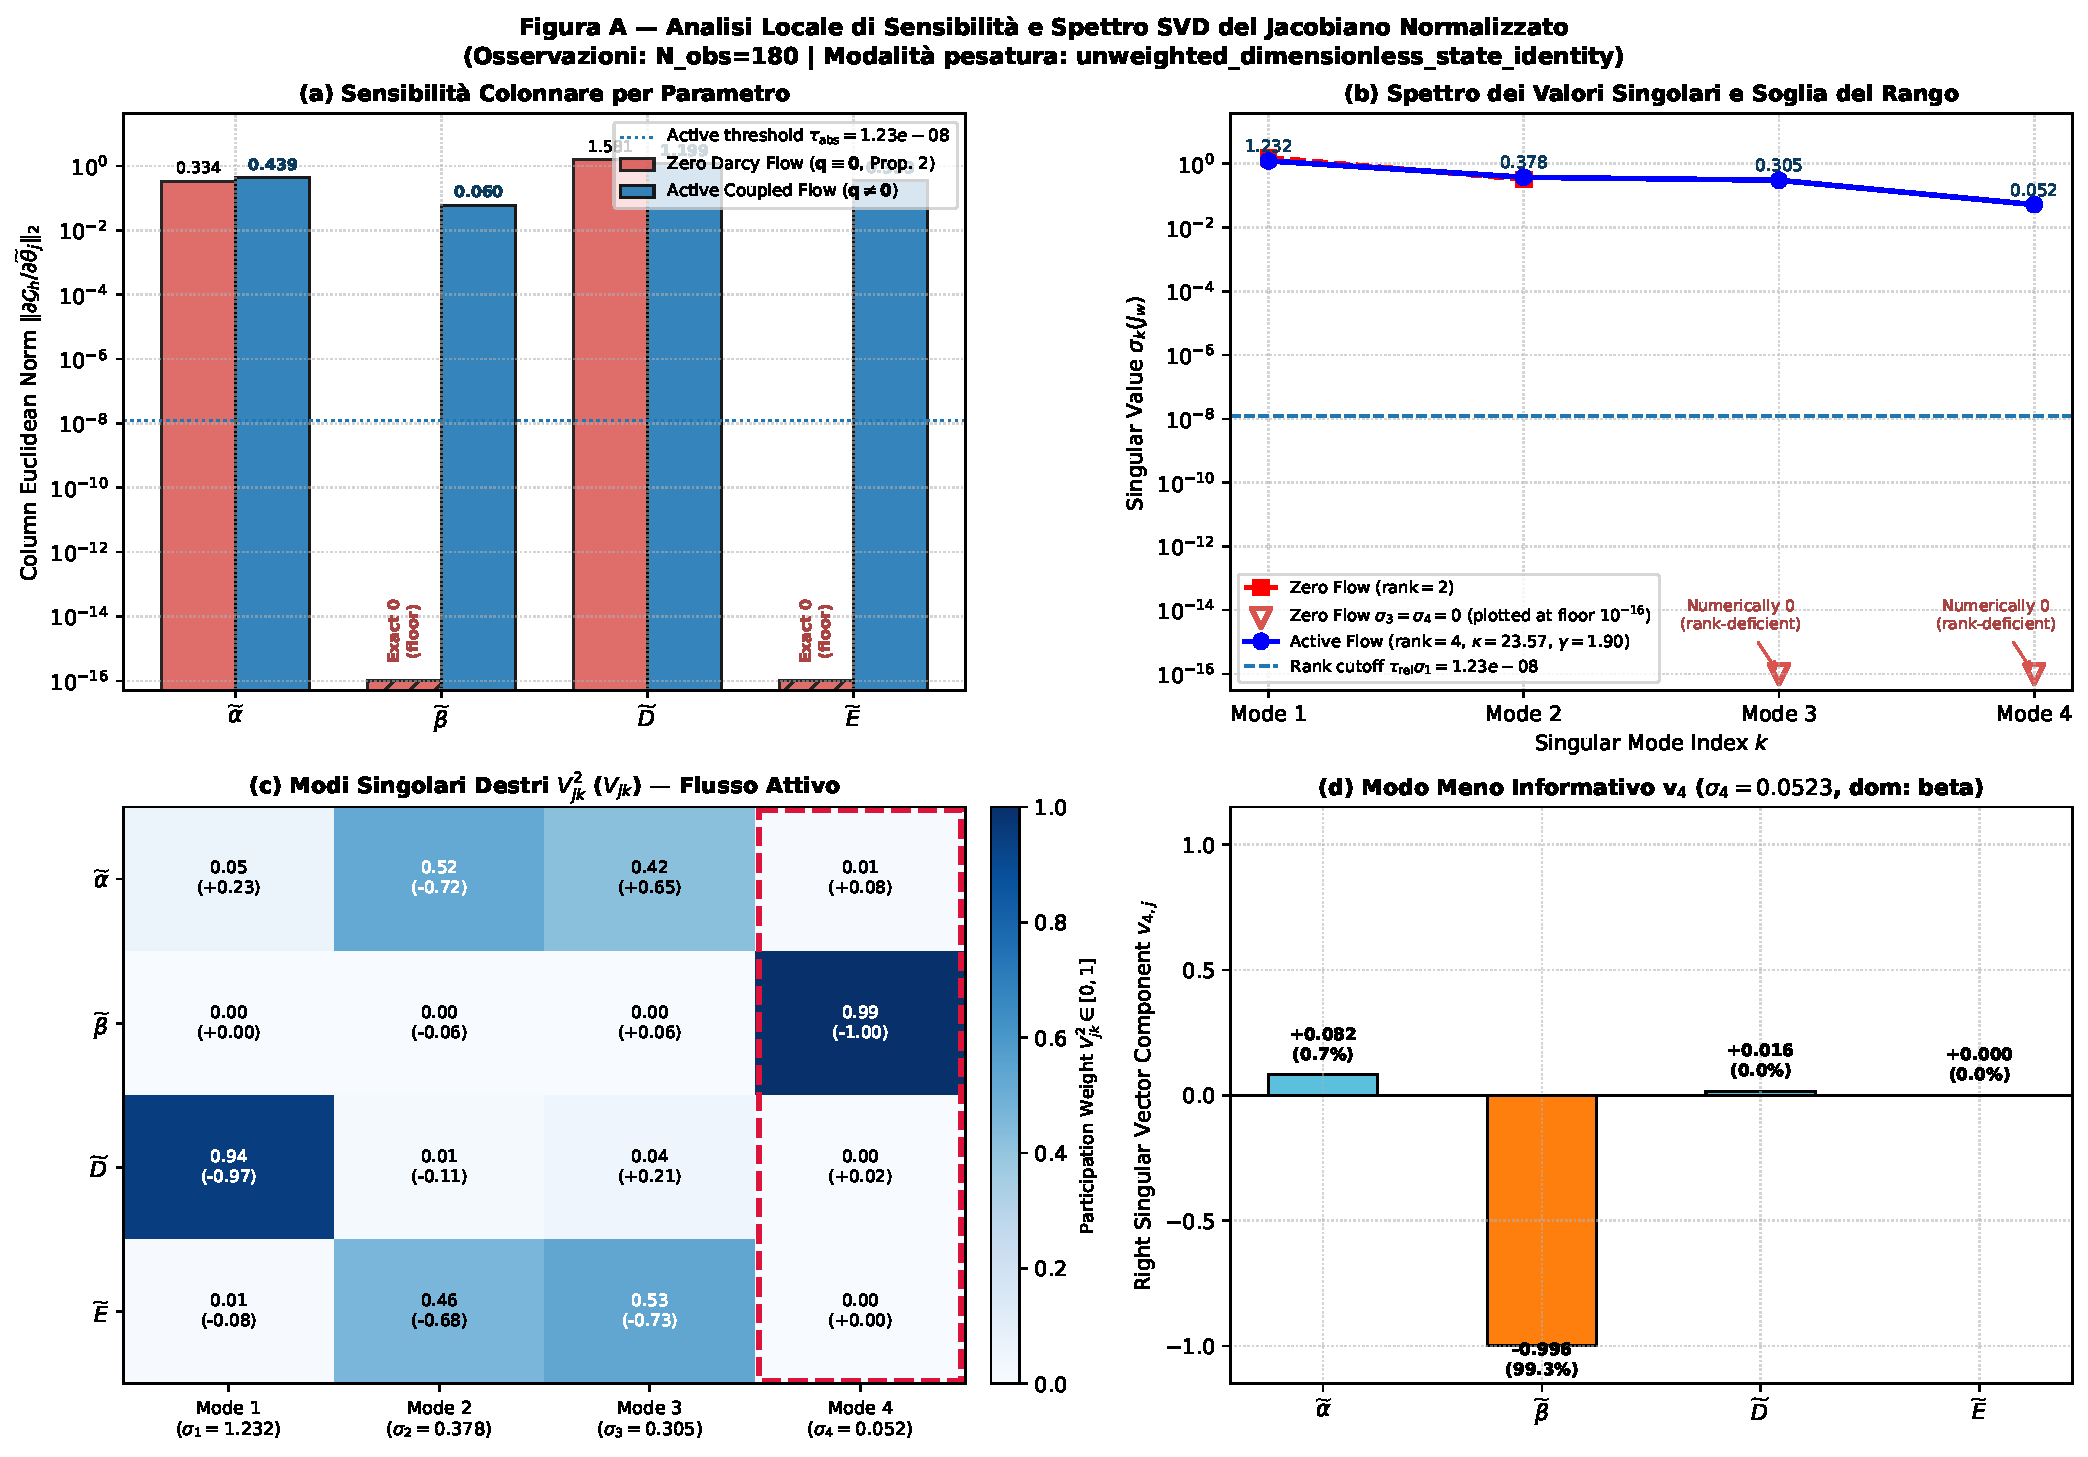
\includegraphics[width=0.94\textwidth]{paper/fig06_sensitivity_and_svd.pdf}
\caption{Diagnostica del Jacobiano osservativo normalizzato: degenerazione esatta nel protocollo a flusso nullo e rango pieno nel protocollo con flusso attivo. L'analisi è locale e non pesata da una covarianza clinica empirica.}
\label{fig:identifiability}
\end{figure*}

Le curve one-at-a-time, che variano un parametro alla volta mantenendo gli altri a $\tht^\dagger$, non includono il compensarsi simultaneo dei parametri. I profili ottimizzati, invece, riottimizzano gli altri parametri ma sono scansioni numeriche del funzionale sintetico e non profili di verosimiglianza statistici. I dettagli sono nell'Appendice C.

\subsection{Profili ottimizzati rispetto a \texorpdfstring{$\beta$}{beta} e sensibilità alla discretizzazione}

Per distinguere la sensibilità del termine dati dall'effetto della penalizzazione, sono stati calcolati due profili numerici bidirezionali su 15 valori di $\beta\in[0.15,0.90]$: $\Phi_{\rm data}(\beta)=\min_{\alpha,D,E}J_{\rm data}$ e $\Phi_{\lambda}(\beta)=\min_{\alpha,D,E}J_{\rm total}$. La scansione è stata eseguita sulla discretizzazione inversa $N=16$, $M=80$, mantenendo fisso il target sintetico e senza utilizzare $\boldsymbol\theta^\dagger$ nell'ottimizzazione. Il minimo campionato di $\Phi_{\rm data}$ si trova in $\beta=0.4500$; quello di $\Phi_{\lambda}$ in $\beta=0.479143$. Le regioni campionate entro il 25\% del minimo sono rispettivamente $[0.425,0.450]$ e $[0.425,0.525]$. La maggiore ampiezza del secondo intervallo è coerente con l'interazione tra il termine dati e la regolarizzazione: il prior normalizzato $\widetilde\beta_0=0.5$ corrisponde a $\beta=0.525$ nei limiti fisici adottati e contribuisce quindi a spostare il minimo del funzionale totale.

\begin{table*}[t]
\centering
\caption{Sintesi dei profili ottimizzati campionati rispetto a $\beta$ sulla discretizzazione inversa $N=16$, $M=80$. Gli intervalli sono insiemi di punti della griglia entro la soglia indicata; non sono intervalli di confidenza statistici.}
\label{tab:beta-profiles}
\small
\begin{tabular}{lcccc}
\toprule
Profilo & $\beta$ al minimo campionato & Valore minimo & Regione entro $+10\%$ & Regione entro $+25\%$\\
\midrule
$\Phi_{\rm data}$ & $0.450000$ & $3.4581\times10^{-7}$ & $[0.450,0.450]$ & $[0.425,0.450]$\\
$\Phi_{\lambda}$ & $0.479143$ & $4.4657\times10^{-6}$ & $[0.450,0.500]$ & $[0.425,0.525]$\\
\bottomrule
\end{tabular}
\end{table*}

Le scansioni forward e backward individuano lo stesso valore campionato di $\beta$ per entrambi i profili. Tuttavia, alcuni punti della griglia hanno esaurito il budget interno per direzione: 13/15 punti backward convergono per il profilo dati e 14/15 per ciascuna direzione del profilo regolarizzato. La concordanza dei minimi campionati è dunque una verifica di consistenza numerica, non una dimostrazione di ottimalità globale. Inoltre, $\Phi_{\rm data}$ e $\Phi_{\lambda}$ sono profili del funzionale deterministico usato nell'esperimento, non profili di verosimiglianza statistici.

La sensibilità alla discretizzazione inversa è stata verificata riutilizzando lo stesso target sintetico $N=32$, $M=160$ e confrontando $N=16$, $M=80$ con $N=24$, $M=120$. Sulla griglia locale comune di $\beta$, il minimo campionato del profilo dati si sposta da $0.4500$ a $0.4375$; le stime dei parametri di disturbo $(\alpha,D,E)$ al minimo restano vicine. Il costo al parametro vero diminuisce di un fattore 2.22 e il minimo del profilo campionato di un fattore 3.53 passando alla discretizzazione più fine. Questa variazione documenta la sensibilità del funzionale all'errore di discretizzazione; non è, da sola, una prova di convergenza del problema inverso.

\begin{table*}[t]
\centering
\caption{Sensibilità del profilo dati alla discretizzazione inversa. I minimi sono minimi campionati sulla griglia locale comune, non minimi globali certificati.}
\label{tab:beta-mesh-sensitivity}
\small
\begin{tabular}{lccccc}
\toprule
Griglia inversa & $J_{\rm data}(\boldsymbol\theta^\dagger)$ & Residuo rel. & $\beta_{\min}$ & $\min\Phi_{\rm data}$ & $(\widehat\alpha,\widehat D,\widehat E)$\\
\midrule
$(16,80)$ & $6.2194\times10^{-7}$ & $1.9373\times10^{-3}$ & $0.4500$ & $3.4581\times10^{-7}$ & $(0.7003,0.07932,2.4878)$\\
$(24,120)$ & $2.8055\times10^{-7}$ & $1.3012\times10^{-3}$ & $0.4375$ & $9.8005\times10^{-8}$ & $(0.7007,0.07937,2.5097)$\\
\bottomrule
\end{tabular}
\end{table*}

\subsection{Twin experiments senza rumore: budget esteso}

La campagna senza rumore comprende tre run CPSO con budget pianificato di 600 valutazioni FEM, selezionate dagli artefatti preesistenti senza rieseguire l'ottimizzazione. La soluzione con il valore più basso osservato di $J_{\rm total}$ è la run con seed 20261018, che restituisce $\widehat{\boldsymbol\theta}=(0.6956,0.4791,0.07892,2.4805)$ e residuo relativo rispetto al target pulito pari allo $0.192\%$. Le altre due run mostrano una stima di $\beta$ più distante dal valore vero, pur recuperando $\alpha$, $D$ ed $E$ con errori generalmente inferiori a pochi punti percentuali.

\begin{table*}[t]
\centering
\caption{Tre run CPSO senza rumore con budget pianificato di 600 valutazioni FEM. La run selezionata è quella con il valore minimo osservato di $J_{\rm total}$; nessuna run è certificata convergente.}
\label{tab:baseline-600}
\small
\begin{tabular}{rcrrrrrc}
\toprule
Seed CPSO & Selezionata & $\widehat\alpha$ & $\widehat\beta$ & $\widehat D$ & $\widehat E$ & $J_{\rm total}$ & Residuo pulito [\%]\\
\midrule
20261017 & No & 0.7033 & 0.3880 & 0.07952 & 2.4788 & $6.3224\times10^{-6}$ & 0.2118\\
20261018 & Sì & 0.6956 & 0.4791 & 0.07892 & 2.4805 & $4.4668\times10^{-6}$ & 0.1918\\
20261019 & No & 0.6838 & 0.6033 & 0.07755 & 2.4870 & $8.9289\times10^{-6}$ & 0.5524\\
\bottomrule
\end{tabular}
\end{table*}

Tutte le tre run hanno terminato per esaurimento del budget, non per un criterio di convergenza. La dispersione di $\widehat\beta$ (da 0.3880 a 0.6033) è considerevole rispetto a quella degli altri parametri e concorda con la struttura dei profili: nell'intervallo centrale, differenti combinazioni parametriche possono produrre valori del termine dati dello stesso ordine. Il minimo osservato di $J_{\rm total}$ identifica il miglior candidato trovato nella campagna, non dimostra un minimo globale e non quantifica da solo l'incertezza statistica.

\subsection{Robustezza al rumore: dieci realizzazioni sintetiche}

La campagna rumorosa comprende cinque realizzazioni indipendenti a ciascun livello nominale $\eta=0.05$ e $\eta=0.10$, con seed CPSO mantenuto fisso e seed del rumore distinti. Il livello nominale è definito attraverso la scala $L^\infty$ del target, mentre la tabella riporta separatamente il rapporto realizzato $\|\boldsymbol\epsilon\|_2/\|\mathbf y_{\rm clean}\|_2$: quest'ultimo varia dall'8.41\% al 9.49\% per $\eta=0.05$ e dal 15.96\% al 17.95\% per $\eta=0.10$.

\begin{table*}[t]
\centering
\caption{Recupero parametrico nella campagna rumorosa finale. Sono riportate mediana, minimo e massimo empirici su cinque realizzazioni per livello. Con $n=5$, questi riepiloghi descrivono il campione e non costituiscono intervalli di confidenza.}
\label{tab:noisy-median-summary}
\small
\begin{tabular}{cccrcc}
\toprule
$\eta$ nominale & $n$ & Parametro & Valore vero & Stima mediana [min, max] & Errore relativo mediano [min, max] [\%]\\
\midrule
0.05 & 5 & $\alpha$ & 0.70 & $0.7027\ [0.6447,0.7301]$ & $3.94\ [0.38,7.90]$\\
0.05 & 5 & $\beta$ & 0.45 & $0.4020\ [0.3562,0.5192]$ & $15.37\ [8.47,20.85]$\\
0.05 & 5 & $D$ & 0.08 & $0.08064\ [0.07603,0.08758]$ & $4.71\ [0.79,9.47]$\\
0.05 & 5 & $E$ & 2.50 & $2.6127\ [2.2431,3.1846]$ & $10.28\ [0.99,27.38]$\\
\midrule
0.10 & 5 & $\alpha$ & 0.70 & $0.6847\ [0.6272,0.7478]$ & $4.48\ [2.16,10.40]$\\
0.10 & 5 & $\beta$ & 0.45 & $0.4234\ [0.3476,0.4754]$ & $5.91\ [1.23,22.76]$\\
0.10 & 5 & $D$ & 0.08 & $0.07587\ [0.06897,0.08816]$ & $5.95\ [3.15,13.79]$\\
0.10 & 5 & $E$ & 2.50 & $2.2282\ [1.6559,2.7267]$ & $10.87\ [1.53,33.76]$\\
\bottomrule
\end{tabular}
\end{table*}

La Figura~\ref{fig:cpso-final-convergence} mostra la cronologia del miglior costo osservato nelle tre run senza rumore e nelle dieci run rumorose. Gli errori non seguono un andamento monotono rispetto a $\eta$: ad esempio, l'errore mediano di $\beta$ è maggiore nel campione a $\eta=0.05$ rispetto a quello a $\eta=0.10$. Questo comportamento, insieme all'ampiezza degli intervalli min--max di $E$ e $\beta$, impedisce di sostenere che il recupero peggiori in modo regolare con il rumore o che il metodo sia robusto in senso generale. Inoltre, il seed dell'ottimizzatore è fisso nella campagna rumorosa: per separare la variabilità dovuta al rumore da quella intrinseca al CPSO occorrerebbe un disegno fattoriale con più seed dell'ottimizzatore per ciascuna realizzazione.

Tutte le dieci run rumorose hanno esaurito il budget pianificato di 600 valutazioni FEM e nessuna ha ottenuto un certificato di convergenza. La funzione obiettivo usa la covarianza inversa esatta e $\lambda_B=7.2$ calibrato alla scala di riferimento $\eta_{\rm ref}=0.05$. Il bilanciamento fra dati e penalizzazione dipende però dal livello $\eta$: con le normalizzazioni dichiarate nell'Equazione~\ref{eq:weight-ratios}, il valore equivalente è $\lambda_B^{\rm eq}(\eta)=N_{\rm obs}\lambda_A/\eta^2$, quindi $7.2$ per $\eta=0.05$ e $1.8$ per $\eta=0.10$. Il protocollo eseguito mantiene invece $\lambda_B=7.2$ in entrambi i gruppi; rispetto al bilanciamento equivalente, la penalizzazione ha quindi peso relativo quattro volte maggiore nel gruppo $\eta=0.10$. I risultati descrivono pertanto la campagna effettivamente eseguita, nella quale cambiano sia il rumore sia il rapporto fra termine dati e regolarizzazione, e non isolano l'effetto del rumore. I valori grezzi di $J_{\rm data}$ ai due livelli non vanno confrontati come se fossero sulla stessa scala. I dettagli per run e l'audit del funzionale sono riportati nelle Appendici~\ref{app:noise} e~\ref{app:objective}.

\begin{figure*}[!t]
\centering
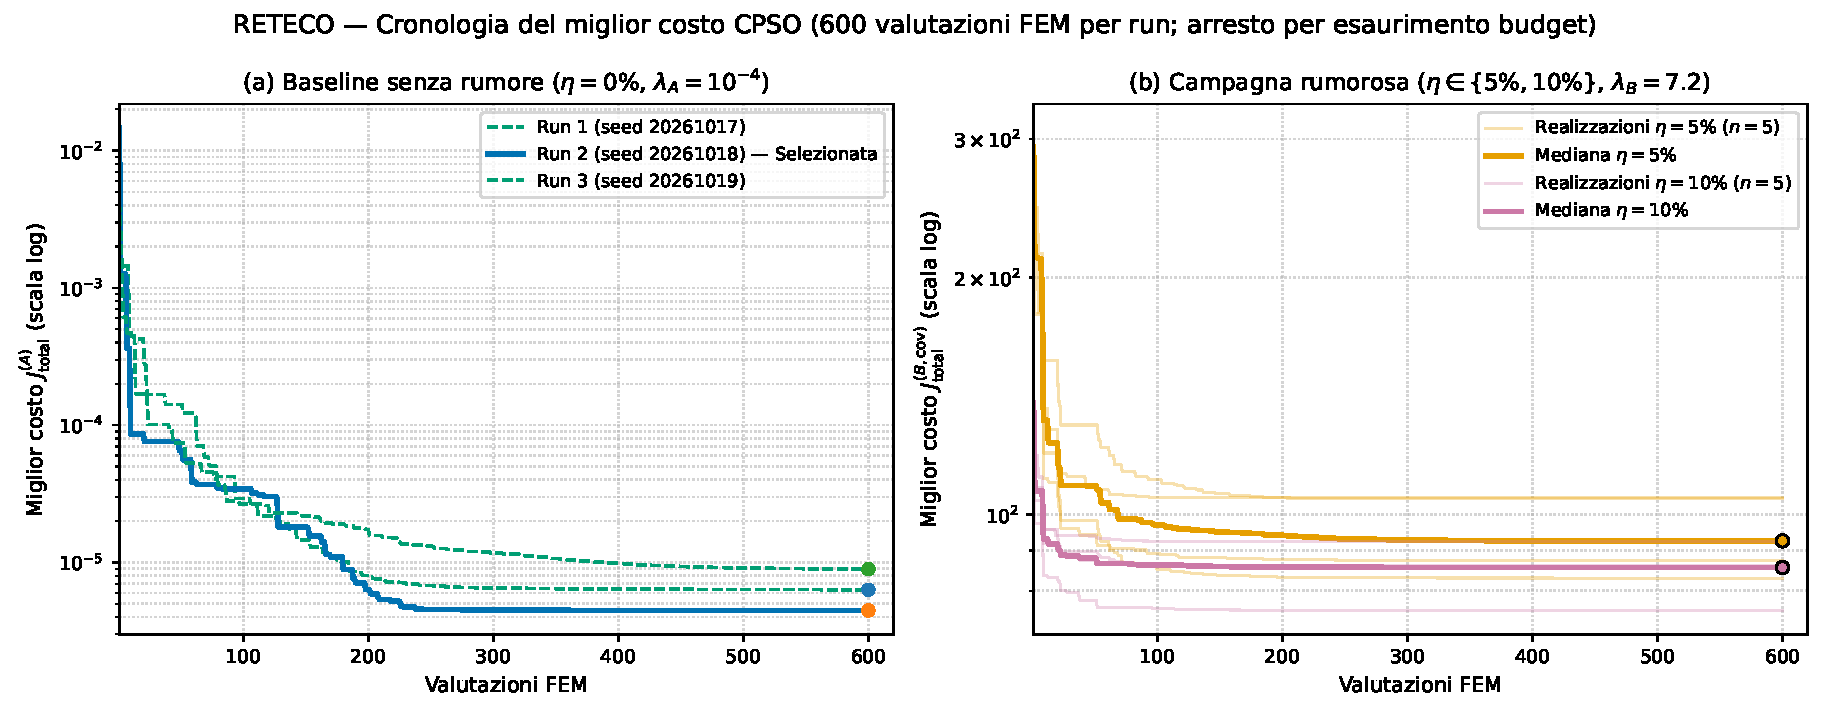
\includegraphics[width=0.98\textwidth,trim=0pt 0pt 0pt 25pt,clip]{paper/fig07_final_cpso_convergence.pdf}
\caption{Cronologia del miglior valore osservato del funzionale obiettivo durante le valutazioni FEM. Il pannello (a) mostra le tre run della baseline senza rumore con pesatura deterministica (Mode A); il pannello (b) mostra le dieci run rumorose con pesatura a covarianza inversa (Mode B covariance), insieme alle mediane empiriche per livello. Le ordinate hanno scale distinte e rappresentano funzionali pesati diversi: i valori assoluti tra pannelli e tra livelli di rumore non sono direttamente confrontabili. Tutte le run terminano per esaurimento del budget; un plateau della curva non costituisce, da solo, una certificazione di convergenza. Il ritaglio LaTeX rimuove soltanto l'intestazione interna con il nome del progetto; il PDF sorgente non è stato modificato.}
\label{fig:cpso-final-convergence}
\end{figure*}
\FloatBarrier

\subsection{Interpretazione della pesatura e limiti della campagna}

La diagnostica dei modi di pesatura conferma che la normalizzazione del termine dati interagisce con $\lambda$. Per il parametro vero sintetico e il livello nominale del 10\%, il termine $J_{\rm data}$ vale $4.119\times10^{-3}$ con la pesatura deterministica, $0.4119$ con la pesatura noise-weighted mean e $74.144$ con la covarianza inversa esatta. Questi valori sono una verifica di scala del funzionale, non una comparazione di prestazioni dell'ottimizzatore. Non è stata eseguita una campagna comparativa a budget equivalente con altri algoritmi; il manoscritto non rivendica quindi superiorità del CPSO.
